\documentclass[12pt,letterpaper]{article}

\usepackage{pslatex}
\usepackage{apacite}
\usepackage{url}
\usepackage{graphicx}
\usepackage{todonotes}
\usepackage{comment}

\usepackage{lineno}
\linenumbers

\usepackage[margin=1in]{geometry}


\usepackage[T1]{fontenc}
\usepackage[utf8]{inputenc}
%\usepackage{tgbonum}
%\usepackage{lmodern}
\usepackage{palatino}

\renewcommand\bibliographytypesize{\small}

\newcommand{\andrew}[1]{\textcolor{magenta}{\bf [Andrew: #1]}}
\newcommand{\rdh}[1]{\textcolor{red}{\bf [Robert: #1]}}


\title{Emergent Collective Sensing\\ in Human Groups:\\Supplementary Materials}

\author{
Robert Hawkins (rdhawkins@princeton.edu)\thanks{Department of Psychology, Princeton University}\\
Andrew M. Berdahl (berdahl@uw.edu)\thanks{School of Aquatic and Fishery Sciences, University of Washington}\\
Alex ``Sandy'' Pentland (pentland@mit.edu)\thanks{MIT Media Lab}\\
Noah D. Goodman (ngoodman@stanford.edu)\thanks{Department of Psychology, Stanford University}\\
Joshua B. Tenenbaum (jbt@mit.edu)\thanks{Department of Brain and Cognitive Sciences, Massachusetts Institute of Technology}\\
P. M. Krafft (p.krafft@oii.ox.ac.uk)\thanks{Oxford Internet Institute, University of Oxford}
}

\date{}
\begin{document}


\maketitle
\vspace{-2em}

\renewcommand{\thesection}{S\arabic{section}}
\renewcommand{\thefigure}{S\arabic{figure}}
\renewcommand{\thetable}{S\arabic{table}}

\setcounter{section}{0}
\setcounter{figure}{0}
\setcounter{table}{0}


\section*{Acknowledgments}

\small

This material is based upon work supported by the National Science
Foundation Graduate Research Fellowship under Grant No. 1122374 to PK
and Grant No. DGE-114747 to RXDH. Any opinion, findings, and
conclusions or recommendations expressed in this material are those of
the authors(s) and do not necessarily reflect the views of the
National Science Foundation.  This material is based upon work
supported by the Center for Minds, Brains and Machines (CBMM), funded
by NSF STC award CCF-1231216.
Special thanks to Colin Torney for providing the code to make the score field gradients, to Hongbo Fang for assisting in validating our qualitative coding, and Robert Goldstone for helpful feedback on the interpretation of our results.


\section*{Ethics}

\small

The research was reviewed and approved by the MIT Committee on the Use of Humans as Experimental Subjects (COUHES), Protocol \#1509172301, as well as the Oxford Internet Institute Departmental Research Ethics Committee (DREC), CUREC 1A Research Ethics Approval Ref Number SSH\_OII\_CIA\_20\_002.



\section*{Competing Interests}

\small

The authors declare no competing interests.


\section*{Data Accessibility}

\small

Data, experiment code, and analysis code are available at \url{https://github.com/hawkrobe/fish}.

\section*{Author Contributions}

\small

RH, PK, AP, NG, and JT formulated  the study. RH and PK designed the experiments, implemented the experiments, and analyzed the data. RH, PK, and AB wrote the manuscript. All authors gave final approval for publication and agree to be held accountable for the work performed therein.

\section*{Appendix A: Behavioral Model}

The trends we observe suggest a potential set of behavioral mechanisms
that participants may be using in our task.  We propose that each
participant chooses an exploring, exploiting, or copying state based on the following
rules:
\begin{enumerate}
\item
  If the participant is in a high scoring area, the participant will remain in that area
  exploiting.
\item
  If the participant is in a low scoring area and the participant perceives another
  person as possibly having a higher score, the participant may choose to
  copy that person.
\item
  Otherwise the participant will explore independently.
\end{enumerate}

This model displays intriguing collective behavior in the score fields that have a smoothly moving high scoring region.
When any individual finds a high scoring area, that participant will attract the
other participants to that location by exploiting.  Then such slowly evolving environments, when all the
participants are together in a group exploiting a particular area, one of
the participants will receive a lower score as the score field shifts.  This
participant will then either move closer to the others who are still
exploiting or will shift to an exploring state.  If that participant starts
exploring but doesn't find any high scoring locations, the participant will return
to the group if the group is still exploiting.  If that participant does
find a new high scoring area, though, the participant will start exploiting that
area.  The rest of the group will then follow after the highest
scoring region shifts to where the exploiting participant is.  This
mechanism creates a kind of gradual crawling that effectively tracks
the moving score field.  Thus, by using this mechanism participants are
improving both their own performances directly and also that of the
entire group by participating in this process of emergent collective
sensing.  An example of this process occurring in participant gameplay
is shown in Figure \ref{fig:example}, and in our Supplementary Videos.

\section*{Appendix B: Experiment 1 methods}

The virtual game environment measured 480 pixels in width and 285 pixels in height.
Avatars were represented by triangles that were 10 pixels in length and 5 pixels in width, rotated to the direction the avatar is facing. 
The avatars automatically moved forward at a constant velocity of 17 pixels per second if no buttons were pressed, but instantaneously increased to a constant velocity of 57 pixels per second for the duration of time that the ``a" key was held down and decreased to 0 pixels per second for the duration of time the "s" key was held down. 
Locations were updated every 125 milliseconds.
To discourage inactivity, participants also received 2/3 of a point for each second they were actively participating in the game.
For any moment when an avatar was touching a wall, we displayed a large warning message and set the participant's current score to zero so that they stopped accumulating points.

We generated score fields by first initializing a circular region with a diameter of 50 pixels at a random location on the playing area. 
Inside this region, the score was set to 1.
Outside this region, the score was set to 0.
We then moved this region along a straight line to a randomly chosen target location within the playing area at a speed of 17 pixels per second.
Once it reached this location, we selected another target location, and repeated the process for the duration of the experiment.

After agreeing to participate in our experiment, participants were presented with a set of instructions describing the mechanics of the game, using a cover story framing the game as a search for the ``magical bonus region" (see GitHub repository).  
The participants were informed about the dynamics of the underlying score field and also explicitly informed that ``There is no competition between players; the magical region is not consumed by players. It simply changes location over time." 
Participants were not explicitly instructed or suggested to cooperate or coordinate with each other.

Participants would wait for up to 5 minutes or until the pre-assigned number of other participants joined.
While in the waiting room, participants could familiarize themselves with the controls of the game.  Participants were not shown any score in
the waiting room unless the participant was against a wall, in which
case the border of the playing region would turn red and a warning appeared on screen.  All participants spent at least one minute in the waiting room to help ensure familiarity with the controls before starting the game. 

Both in the waiting room and the actual game, participants were removed for inactivity if we detected that they had switched to another browser tab for more than 30 seconds total throughout the game or if the participant's avatar was moving into a wall for 30 consecutive seconds.  
We also removed participants if their ping response latencies were greater than 125ms for more than 75 seconds in total throughout the game.  
To minimize disruption of large groups, we allowed multi-participant games to continue after a participant disconnected or was removed, as long as at one or more participants remained.

We paid participants 75 cents for completing our instructions and comprehension checks, and the participants could receive a bonus of up to \$1.25 during the five minutes of gameplay. Each point in the game corresponded to \$0.01 of bonus. Each participant was also paid 15 cents per minute for any time spent in the waiting room, minus any time that participant spent moving into a wall.  These numbers were chosen so that the participants were expected to receive at least a wage of \$9 per hour for the totality of their time active in the
experiment.

We implemented this experiment using the MWERT framework \cite{hawkins_conducting_2014}, which uses a stack of recent web technologies capable of handling the challenges of real-time, multi-participant web experiments, including Node.js, the Socket.io module, and HTML5 canvases.  

\section*{Appendix C: Experiment 2}

\subsection*{Methods}

To acclimate participants to the task environment, each game began with four one-minute long practice rounds. 
In the first and third practice rounds, the score field was \emph{visible} to the participant so they could observe its dynamics.
In the second and fourth practice rounds, the score field was invisible to the participants, as in Experiment 1. 
Additionally, we randomized participants into two different groups, who practiced with different score field dynamics. 
In a ``wall-following'' pattern, the high scoring region moved contiguously along the walls of the playing area. 
In a ``random-walk'' pattern, the high scoring region slowly drifted, as in Experiment 1, from one random location to another within the playing region.
Because we did not observe substantial differences in participant behavior depending on the score field dynamics observed during the practice phase, we collapsed over this factor in our analyses.

\subsection*{Qualitative Coding Results}

For our qualitative analysis, two authors manually coded videos of our 28 participants. We coded for three behavioral signatures --- \emph{selectivity} in copying exploiting bots, \emph{eagerness} in copying other agents, and \emph{independence} in exploration --- on a scale from 0 to 1. \emph{Selectivity} was defined by examining behavior during the distant condition, when the participant was not themselves receiving a reward but another agent was: selectivity was coded as a preference for moving towards agents who were exploiting, as opposed to moving toward agents who were exploring or copying. This behavioral signature marks participants as selectively copying agents who are exploiting the high scoring regions.
\emph{Eagerness} was defined by the same preference for moving toward exploiting agents during the local condition when the participants were themselves receiving a high score, such that their copying behavior was not contingent on their own state. Eager agents copy even when they could be exploiting the high scoring region they have already identified.
Finally, \emph{independence} was defined by reverse-coding a preference for moving towards agents who were \emph{not} stopped, at any point in the task---i.e., indiscriminately copying other agents. This signature primarily captures whether participants were preferentially moving toward other agents during the periods when there was no score field active, thus we interpret low prevalence of this signature as high independence. 
The endpoints of the scale roughly represented the proportion of time the participant spent displaying the behavior in question compared to the potentially available opportunities to do so. 

The two coders achieved a correlation of $r = 0.75$ for selectivity, $r = 0.55$ for eagerness, and $r = 0.60$ for independence. The coders resolved disagreements in our codes by averaging. 
First, we found that a substantial fraction of participants display selective copying behavior and independence (Supplemental Fig. S2). 
%\todo[inline]{rdh: Is it appropriate to use 0.5 as the null threshold? Do we think that midpoint is meaningful, since even lower numbers, e.g. 0.2, were indicative of some level of these signatures? Maybe should be comparing to a null of 0?}
We found that 71\% of participants had an average selectivity rating of at least 0.5, and 86\% had an average independence rating above that level. 
These proportions were significantly greater than 50\% using a two-sided binomial test, $p = 0.036$ and $p = 0.001$, respectively.  
In comparison, only 1 participant (4\%) was coded as eager at that level, which was significantly less than 50\%, $p < 0.001$.
These qualitative results show that participants appeared to selectively copy stopped agents when they themselves were not receiving reward, but otherwise mostly inhibited social influence.

\section*{Appendix D: Experiment 3 methods}

Our criteria for classifying the three states are as follows.
\begin{itemize}
\item \emph{Exploiting} behavior was not trivial for participants since the avatars always move at least at a slow constant velocity. 
Unlike in the previous experiments, where the ``s'' could could be pressed to stop in place, a participant in Experiment 3 could either meander around a particular location or persistently hold down one of the arrow keys while moving at a slow speed, which creates a relatively tight circular motion around a particular location.  
We call this second activity ``spinning'' because of its distinctive appearance.  
We then classify a participant as exploiting if the participant is spinning for 1 second, or if the participant moves at a slow speed for 3 seconds and has not traveled more than two thirds of the possible distance that the participant could have traveled in that time.
The second condition is captures the meandering behavior of individuals who have not discovered how to spin.
\item \emph{Copying} behavior is more difficult to identify, but is likely characterized by directed movements towards other participants. 
We thus classify a participant as copying if they move at the fast speed in a straight line towards any particular other participant for a 500ms window.
We consider a participant to be moving towards another participant if the second participant is within a $60^\circ$ on either side of the first participant's straight-line trajectory.
\item We classify behavior as \emph{exploring} if the participant is neither exploiting nor copying. Thus, a participant will be classified as exploring if that participant is either moving slowly but not staying in the same general location, if the participant is moving quickly but not towards any particular person, or if the participant is moving quickly and turning.
\end{itemize}

\begin{figure}
  \centering
  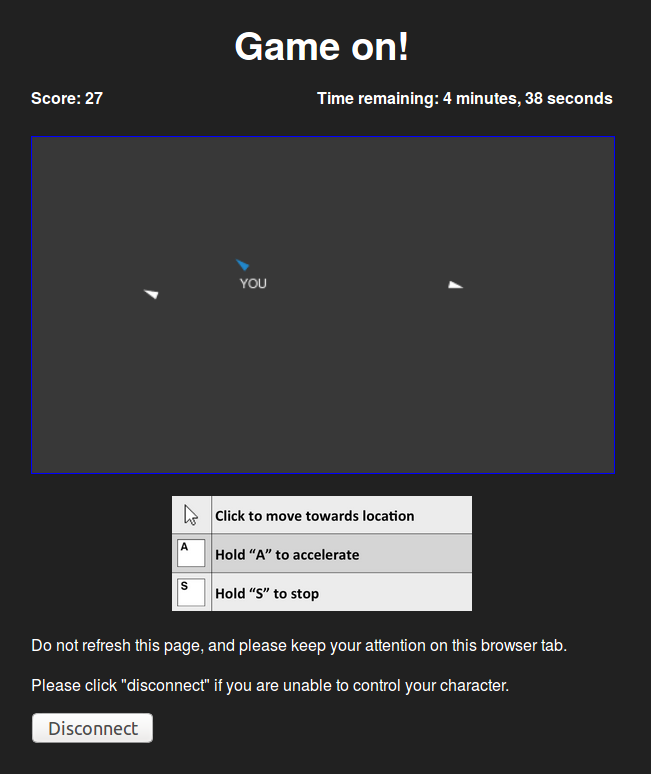
\includegraphics[width=0.45\textwidth]{./figures/experiment-3-no-score}
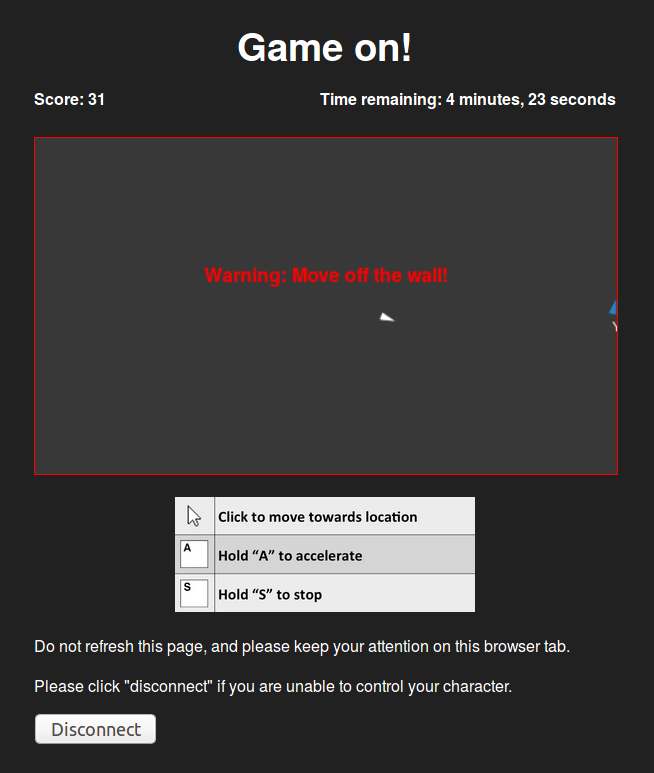
\includegraphics[width=0.45\textwidth]{./figures/experiment-3-wall}
  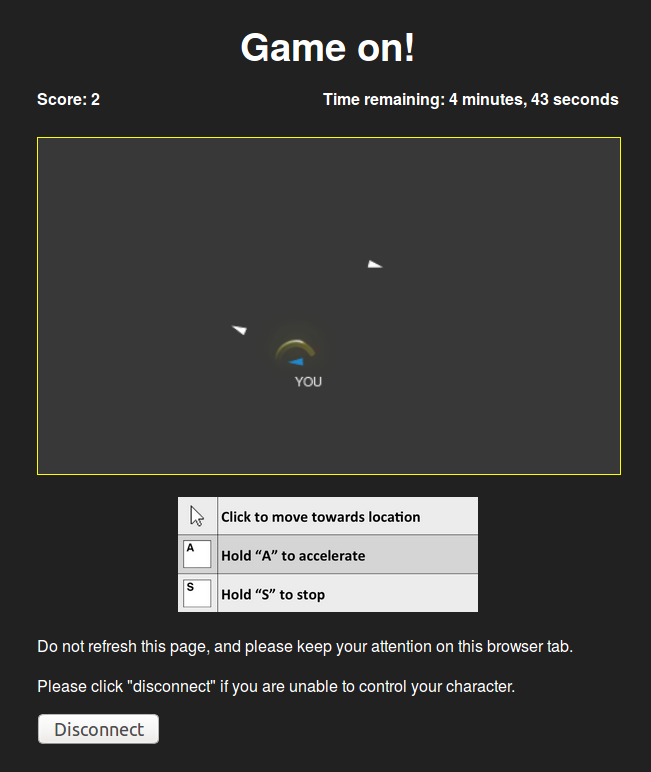
\includegraphics[width=0.5\textwidth]{./figures/experiment-3-score}
  \hspace{0.1cm}
  \caption{Examples of Experiment 1 interface.}
  \label{fig:supplemental_interface}
\end{figure}

\begin{figure}[t!]
    \centering
    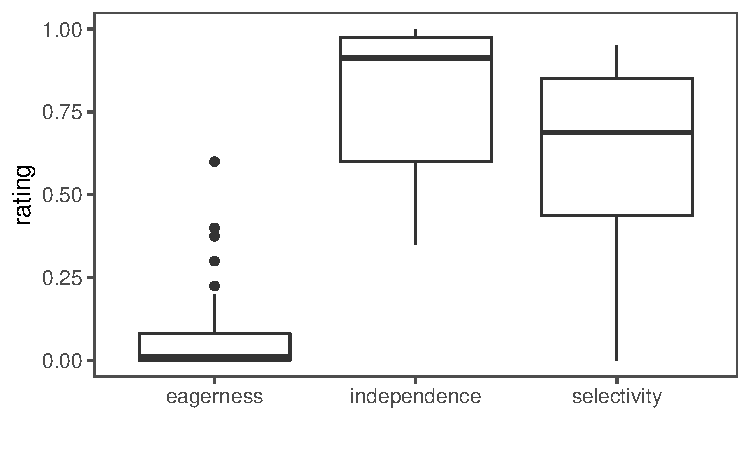
\includegraphics[width=0.9\linewidth]{figures/coding.pdf}
    \caption{Distribution of ratings for three qualitative behavioral properties that were coded from videos in Experiment 2. Participants displayed relatively high levels of selective copying behavior and independent exploration, while eager copying is less common. Center line represents median; box limits represent upper and lower quartiles; whiskers represent 1.5x interquartile range; points represent outliers.}
    \label{fig:selective}
\end{figure}


\begin{figure}[b!]
  \centering
  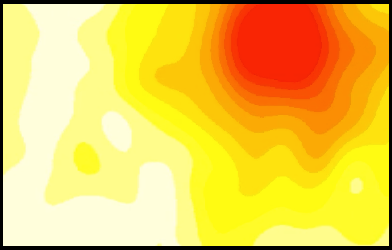
\includegraphics[width=0.4\textwidth]{./figures/easy-field}
  \hspace{0.1cm}
  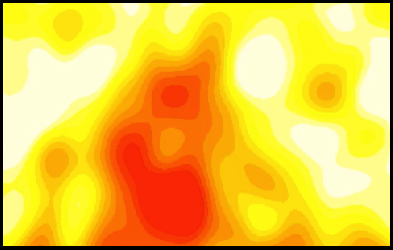
\includegraphics[width=0.4\textwidth]{./figures/medium-field}
  \caption{Example snapshots of score fields from the low noise (left) and high noise (right) conditions used in Experiment 3.  Red areas indicate higher scoring areas.}
  \label{fig:score_exp3}
\end{figure}


\begin{figure*}
\centering
  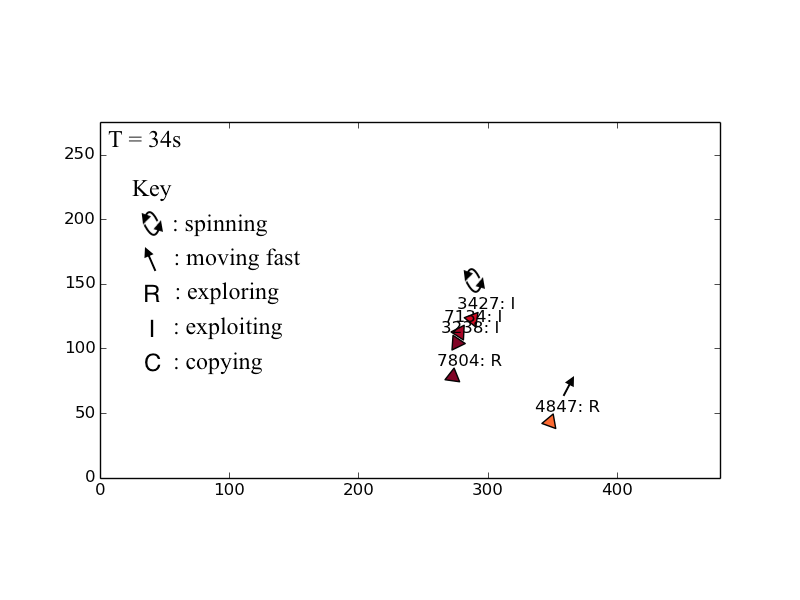
\includegraphics[width=0.45\textwidth,trim=2.5cm 3cm 2cm 3cm,clip]{./figures/pos0274}
  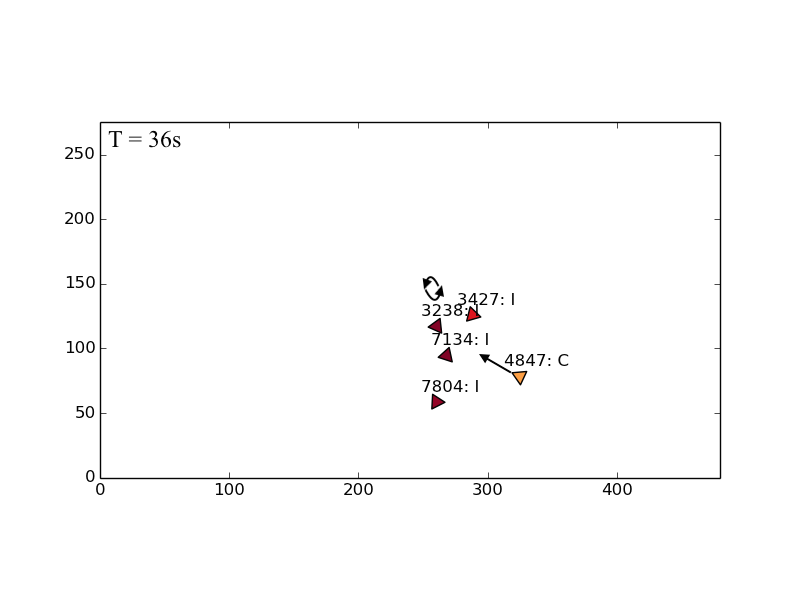
\includegraphics[width=0.45\textwidth,trim=2.5cm 3cm 2cm 3cm,clip]{./figures/pos0285}
  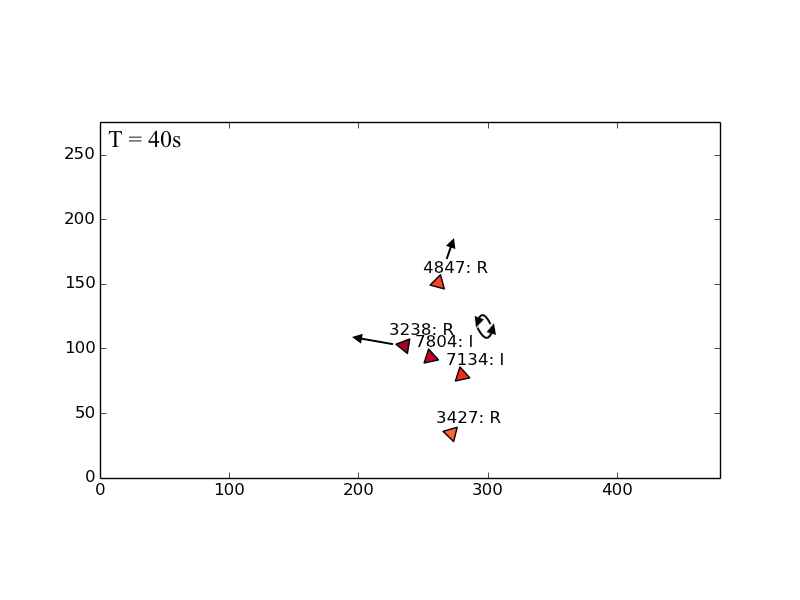
\includegraphics[width=0.45\textwidth,trim=2.5cm 3cm 2cm 3cm,clip]{./figures/pos0323}
  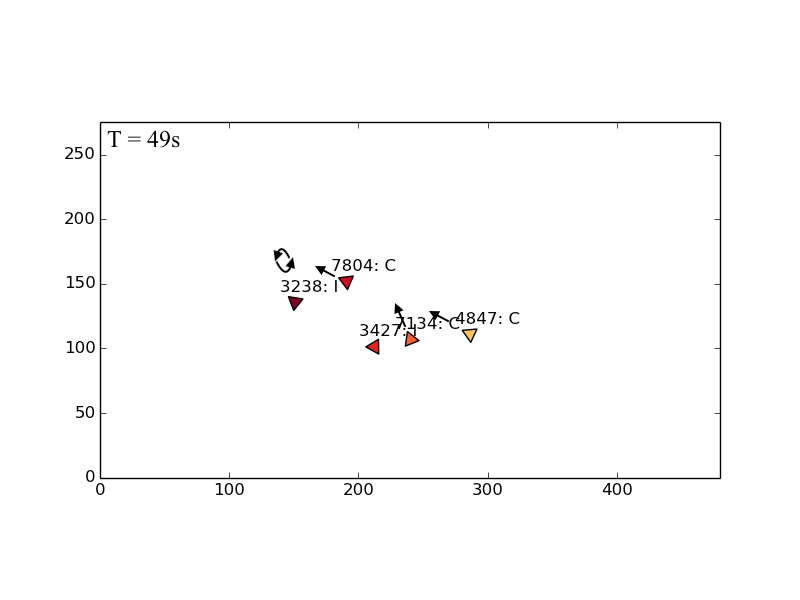
\includegraphics[width=0.45\textwidth,trim=2.5cm 3cm 2cm 3cm,clip]{./figures/pos0394} % 388
  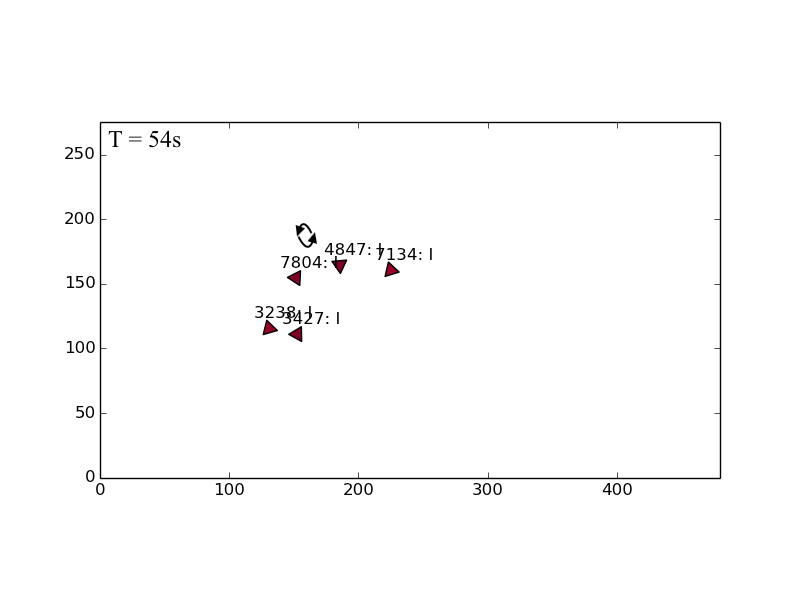
\includegraphics[width=0.45\textwidth,trim=2.5cm 3cm 2cm 3cm,clip]{./figures/pos0435}
  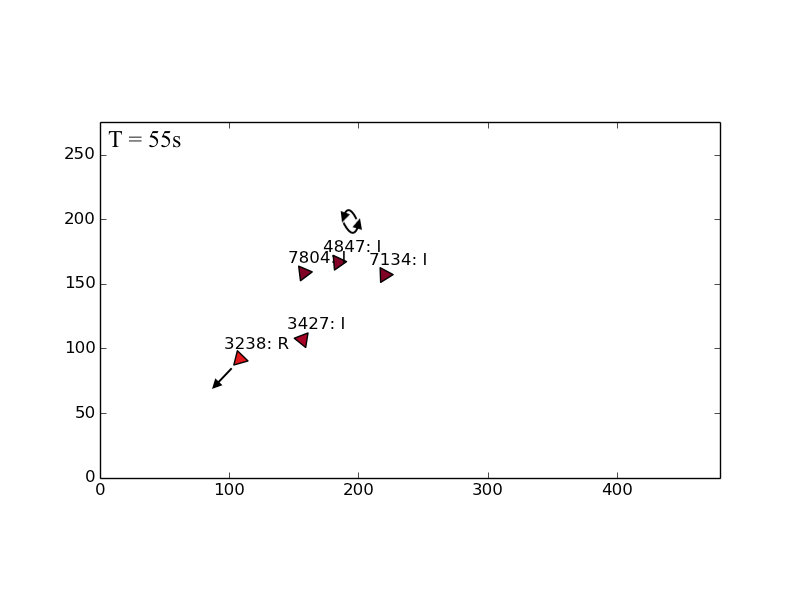
\includegraphics[width=0.45\textwidth,trim=2.5cm 3cm 2cm 3cm,clip]{./figures/pos0441}
  \caption{Reconstructions of actual gameplay in a five-person group
    illustrating both failed exploration leading to intelligent
    copying and successful exploration leading to collective
    movement. Colors indicate the individuals' scores, with red being
    higher and orange/yellow being lower.  The participant labels indicate
    both participant IDs and also the participant states our feature extraction
    procedure inferred.  Other annotations are provided to give a
    sense for the game dynamics.  At $34$ seconds, in the first panel,
    most of the group has converged on exploiting a particular area
    while one individual is exploring independently.  To the right, at
    36 seconds, the exploring individual appears to have failed to
    find a good location and ceases exploring by copying the group.
    At 40 seconds, the final panel in the first row, the score field
    has shifted and some of the group begins exploring while others
    continue to exploit.  By 49 seconds, the first panel in the second
    row, one of the exploring individuals found a good location, and
    other participants have begun to move towards that individual.  At 54
    seconds, the entire group is exploiting the new area.  In the
    final panel, at 55 seconds, the background has shifted enough
    again that one of the individuals begins to explore.}
  \label{fig:example}
\end{figure*}



\begin{figure}
  \centering
  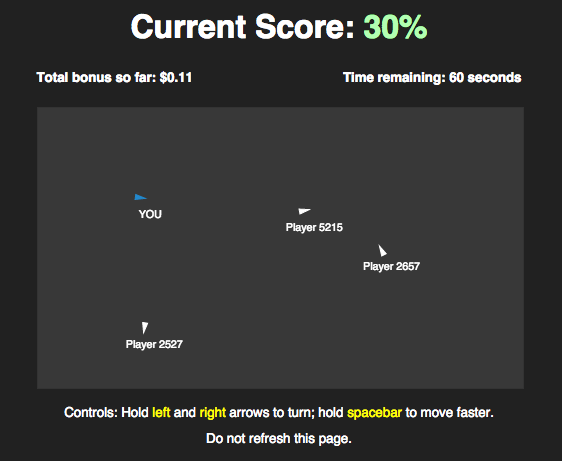
\includegraphics[width=0.9\textwidth]{./figures/interface}
  \caption{Screenshots of the Experiment 3 interface.  The
    score displayed corresponds to the value of the score field at the
    location that the participant's avatar is occupying.}
  \label{fig:exp3_interface}
\end{figure}

\bibliographystyle{apacite}

\setlength{\bibleftmargin}{.125in}
\setlength{\bibindent}{-\bibleftmargin}

\small{
  \bibliography{couzin}
}

\end{document}
